%% Supplemental Material for preprint.tex. Build after the main text, whose labels it reads:
%%   pdflatex supplement ; bibtex supplement ; pdflatex x2
\documentclass[aps,prx,twocolumn,superscriptaddress,nofootinbib,amsmath,amssymb,floatfix]{revtex4-2}

\usepackage{amsmath,amssymb,amsfonts,bm}
\usepackage{braket}
\usepackage{graphicx}
\usepackage{booktabs}
\usepackage{multirow}
\usepackage{siunitx}
\usepackage{xcolor}
\usepackage{xr-hyper}
\usepackage[colorlinks=true,linkcolor=blue,citecolor=blue,urlcolor=blue]{hyperref}
\externaldocument[M-]{preprint}
\def\UrlBreaks{\do\/\do\-\do\.}

\graphicspath{{figures/}}

\sisetup{detect-all=true,range-phrase={--},range-units=single}

% ---- convenience macros -------------------------------------------------
\newcommand{\Ntgt}[2]{N(#1,#1,#2)}
\newcommand{\Ltot}{L_{\mathrm{tot}}}
\newcommand{\Hod}{\hat{H}_{\mathrm{od}}}
\newcommand{\Utgt}{U_{\mathrm{target}}}
\newcommand{\Fbar}{\overline{F}}
\newcommand{\snoise}{\sigma_{\mathrm{noise}}}
\newcommand{\strain}{\sigma_{\mathrm{train}}}
\newcommand{\Tsyn}{T_{\mathrm{syn}}}
\newcommand{\ns}{\,\mathrm{ns}}
\newcommand{\MHz}{\,\mathrm{MHz}}

\begin{document}

\title{Supplemental Material for ``Robust analog two-qubit gates from deep reinforcement learning:\\
an independent reproduction and family-resolved assessment''}

\author{Francesco Giuseppe Minisini}
% \email{fg.minisini@gmail.com}
\affiliation{EPFL, Switzerland}
\author{Davide Emilio Galli}
% \email{davide.galli@unimi.it}
\affiliation{Università Degli Studi di Milano, Italy}
\author{Morten Hjort Jensen}
% \email{Morten-Hjort-Jensen@uio.no}
\affiliation{University Of Oslo, Norway}

\date{\today}

\maketitle

\renewcommand{\thesection}{S\arabic{section}}
\renewcommand{\thesubsection}{\arabic{subsection}}
\renewcommand{\theequation}{S\arabic{equation}}
\renewcommand{\thefigure}{S\arabic{figure}}
\renewcommand{\thetable}{S\arabic{table}}

This document collects material that supports the main text: the derivation of the leakage bound
(Sec.~S1), algorithmic details (Sec.~S2), the complete configuration of every run (Sec.~S3), the sweeps
that fix the free parameters (Sec.~S4), the horizon sweep of the direct optimizer (Sec.~S5), the two
family sweeps target by target (Sec.~S6) and further remarks on the relation to hardware (Sec.~S7).
Section, equation, figure and table numbers without the prefix S refer to the main text.

\section{The TSWT coherent leakage bound}
\label{app:tswt}

We summarize the derivation of Eq.~\eqref{M-eq:leakbound}. Starting from the decomposition
Eq.~\eqref{M-eq:decomp} in the regime $\epsilon/\Delta\ll1$, one seeks an anti-Hermitian generator
$\hat S(t)=\epsilon\hat S_1+\epsilon^2\hat S_2+\dots$ such that the transformed Hamiltonian
Eq.~\eqref{M-eq:tswt} is block-diagonal to the desired order. Order by order, the block-off-diagonal
components must satisfy
\begin{equation}
[\hat H_0,\hat S_1]=-\hat H_2,\qquad
[\hat H_0,\hat S_2]=-\bigl([\hat H_1,\hat S_1]-i\dot{\hat S}_1\bigr)_{\mathrm{od}},
\label{eq:generators}
\end{equation}
which are solved elementwise on the off-diagonal blocks by dividing by the subspace energy differences
$E_\alpha-E_{\alpha'}$; the assumption $\epsilon/\Delta\ll1$ is what makes these divisions safe. After
second order the residual block-off-diagonal Hamiltonian is
\begin{equation}
H_{\mathrm{od}}^{(3)}=[\hat H_1,\hat S_2]+\tfrac{1}{3}\bigl[[\hat H_2,\hat S_1],\hat S_1\bigr]-i\dot{\hat S}_2
=O\!\left(\frac{\epsilon^3}{\Delta^2}\right).
\label{eq:hod3}
\end{equation}
The leakage amplitude out of $\Omega_0$ over $[0,T]$ is then an interaction-picture integral of
$\Hod$ against a rapidly oscillating phase $e^{i\int\Delta dt}$. Repeated integration by parts
converts this into boundary terms, which pick up $\|\Hod\|/\Delta$ at $t=0$ and $t=T$, plus a residual
integral controlled by the second derivative of $\Hod$ divided by $\Delta^2$. Collecting these gives
Eq.~\eqref{M-eq:leakbound}.

The two contributions dominate in complementary regimes: for slow, off-resonant modulation the
boundary terms dominate, and for faster on-resonant modulation the derivative term does. This is why
the bound is usable as a single penalty across the operating range rather than only in one limit.

\section{Algorithmic details}
\label{app:algo}

\paragraph*{Environment step.}
Given the current observation and propagator: map the action to physical controls; apply the bandwidth
filter Eq.~\eqref{M-eq:filter}; if stochastic training is enabled, sample Gaussian perturbations for
$g,\delta_{1,2},f_{1,2}$ and $\eta$ and wrap the phases modulo $2\pi$; build $H_t$ from
Eq.~\eqref{M-eq:hrwa}; propagate $U_{t+1}=e^{-iH_t\Delta t}U_t$ by exact diagonalization; update the
leakage estimator with the same, possibly noisy, $H_t$; evaluate the running cost Eq.~\eqref{M-eq:ufo} and
reward $r=-C$; test the stopping
condition (time limit or cost threshold); emit the next observation Eq.~\eqref{M-eq:obs}.

\paragraph*{Incremental leakage estimator.}
At each step: decompose $H_t$ into $H_0,H_1,H_2$; solve Eq.~\eqref{eq:generators} for $S_1$; estimate
$\dot S_1$ from the stored previous value by finite differences; solve for $S_2$; estimate $\dot S_2$;
form $H_{\mathrm{od}}^{(3)}$ from Eq.~\eqref{eq:hod3} and symmetrize; take its spectral norm. The first
and last samples update the boundary contribution; the discrete second derivative, formed from the two
previous stored values, updates the integral contribution. Storing only the two previous states keeps
the estimator $O(1)$ per step.

\paragraph*{TRPO loop.}
Per iteration: collect a batch of stochastic rollouts in parallel workers; compute discounted returns
and generalized advantage estimates~\cite{Schulman2016GAE}; take the KL-constrained policy step
Eq.~\eqref{M-eq:trpo} by conjugate gradient with backtracking line search; refit the value network by
regression on the empirical returns; evaluate the deterministic policy in the nominal environment and
store the pulse if it improves on the best so far. Checkpoints and induced pulses are
saved every iteration, so that comparisons can be made at the level of the realized pulse rather than
only at the level of network weights.

\paragraph*{Direct optimizer.}
For each candidate horizon the raw parameters are initialized to zero, which after the $\tanh$ map gives
zero amplitudes and phases $\pi$. Each of the $400$ steps filters the controls, simulates one trajectory
perturbed at $\strain$, evaluates the UFO cost including the leakage bound on that noisy trajectory,
back-propagates, clips the gradient norm at $10$ and takes an Adam step. Section~\ref{M-sec:controllers}
describes how the stored pulse and the horizon are selected.

\section{Complete configuration}
\label{app:config}

Table~\ref{tab:config} collects every setting used. We report per-experiment values rather than a single
idealized configuration, because the runs differ in budget and stopping cost, and the two single-target
agents were trained in two stages.

\begin{table*}[t]
\caption{Complete configuration, as actually run. The four right-hand columns are the two single-target
RL agents (Secs.~\ref{M-sec:single}--\ref{M-sec:robust}), the architecture and UFO-weight sweeps
(Appendix~\ref{app:modelsel}) and the curriculum runtime sweep (Sec.~\ref{M-sec:runtime}); an entry spanning
several columns applies to all of them. Every RL run except the noise-free agent was trained with noise.}
\label{tab:config}
\footnotesize
\begin{ruledtabular}
\begin{tabular}{llcccc}
Quantity & Symbol & Single target & Arch.\ sweep & Weight sweep & Curriculum \\
\colrule
\multicolumn{6}{l}{\textit{Physical model}}\\
Levels per mode & --- & \multicolumn{4}{c}{$3$}\\
Anharmonicity & $\eta$ & \multicolumn{4}{c}{$-200\MHz$}\\
Control bound & $u_{\max}$ & \multicolumn{4}{c}{$20\MHz$}\\
Filter bandwidth & $B$ & \multicolumn{4}{c}{$10\MHz$}\\
Timestep & $\Delta t$ & \multicolumn{4}{c}{$2\ns$}\\
Max gate duration & $T_{\max}$ & \multicolumn{4}{c}{$180\ns$}\\
Runtime norm. & $T_{\mathrm{norm}}$ & \multicolumn{4}{c}{$60\ns$}\\
Target & --- & \multicolumn{3}{c}{$\Ntgt{2.2}{\pi/2}$} & $\alpha=0,0.157,\dots,3.14$\\
\colrule
\multicolumn{6}{l}{\textit{UFO weights}}\\
Fidelity, leakage & $\chi$, $\beta$ & $10$, $10$ & $10$, $10$ & $\{5,10,20\}$, $10$ & $10$, $10$\\
Boundary & $\mu$ & $0.2$ & $0.2$ & $\{0.1,0.2,0.4\}$ & $0.2$\\
Runtime & $\kappa$ & $0.1$ & $0.1$ & $\{0.05,0.1,0.2,0.4\}$ & $0.1$\\
\colrule
\multicolumn{6}{l}{\textit{TRPO}}\\
Hidden sizes & --- & $(64,32,32)$ & five layouts & $(64,32,32)$ & $(64,32,32)$\\
Trust region & $\delta_{\mathrm{KL}}$ & \multicolumn{4}{c}{$0.01$}\\
Discount, GAE parameter & $\gamma_{\mathrm{RL}}$, $\lambda$ & \multicolumn{4}{c}{$0.99$, $0.97$}\\
CG iterations, damping & --- & \multicolumn{4}{c}{$10$, $0.1$}\\
Value lr, epochs & --- & \multicolumn{4}{c}{$10^{-3}$, $50$}\\
Initial exploration & $\log\sigma_0$ & $-0.5$ & $-1.0$ & $-1.0$ & $-0.5$\\
Episodes per batch & --- & $10\,000$\footnotemark[1] & $5000$ & $10\,000$ & $4000$\\
Policy iterations & --- & $100+15$ / $100+5$\footnotemark[1] & $20$ & $5$ & ${\le}150$ per target\\
Stopping cost & $C_{\mathrm{term}}$ & $0.40$, then $0.30$\footnotemark[1] & $0.40$ & $0.15$ & $0.40$\footnotemark[2]\\
Training noise & $\strain$ & $0$ / $1\MHz$\footnotemark[3] & $1\MHz$ & $1\MHz$ & $1\MHz$\\
Seeds & --- & $1$ & $1,2,3$ & $1,2$ & $2$\\
\colrule
\multicolumn{6}{l}{\textit{direct optimizer (single target and family sweep)}}\\
Iterations per horizon, lr & --- & \multicolumn{4}{c}{$400$, $0.03$; one deterministic initialization; seed $2$}\\
Horizon grid & --- & \multicolumn{4}{c}{$40$--$180\ns$, step $10\ns$}\\
Training noise & $\strain$ & \multicolumn{4}{c}{$1\MHz$, one noisy trajectory per step}\\
Family targets & --- & \multicolumn{4}{c}{$\alpha=0,0.1,\dots,3.1$ and $\pi$}\\
\colrule
\multicolumn{6}{l}{\textit{Robustness evaluation}}\\
Dense grid & $\snoise$ & \multicolumn{4}{c}{$0.1$--$3.5\MHz$, step $0.001\MHz$, $60$ samples; EWMA spans $50$ / $80$}\\
Matched trajectories & $\snoise$ & \multicolumn{4}{c}{$11$ values in $0.1$--$3.5\MHz$, $200$ samples each}\\
Closed-loop test & $\snoise$ & \multicolumn{4}{c}{$1\MHz$, $100$ samples}\\
\end{tabular}
\end{ruledtabular}
\footnotetext[1]{Both agents: iterations $1$--$100$ with $10\,000$ episodes per batch and
$C_{\mathrm{term}}=0.40$, from the same seed. They then continued with $C_{\mathrm{term}}=0.30$: the
noise-free agent for $15$ iterations with $5000$ episodes per batch, the noise-trained one for $5$
iterations with $10\,000$. The three further pairs of Sec.~\ref{M-sec:matched} (seeds $1$, $2$, $3$) have
the settings of iterations $1$--$100$, with the leakage bound of the noise-trained agents accumulated
from the noise-free controls.}
\footnotetext[2]{Also the advancement threshold. The cold-start target $\alpha=0$ used a hand-tuned
sequence of stopping costs.}
\footnotetext[3]{Nominal / noise-trained agent.}
\end{table*}

\section{Fixing the free parameters}
\label{app:modelsel}

The two sweeps summarized in Sec.~\ref{M-sec:modelsel} were run on the representative target
$\Ntgt{2.2}{\pi/2}$, under a reduced budget and before any production run. Every sweep run is
noise-trained at $\strain=1\MHz$.

\subsection{Actor--critic architecture}
\label{sec:arch}

We swept five hidden-layer layouts of comparable scale, three seeds each, at $20$ policy iterations and
$5000$ episodes per batch (Table~\ref{tab:arch}). Selection was not made on total cost alone, because
a network can reach a favourable cost by trading leakage against fidelity or by settling on an
unnecessarily long pulse; we therefore tracked nominal fidelity, leakage, runtime and robustness at
$\snoise=1\MHz$ simultaneously.

\begin{table}[t]
\caption{Architecture sweep on $\Ntgt{2.2}{\pi/2}$, averaged over three seeds. Best value in each
column in bold.}
\label{tab:arch}
\begin{ruledtabular}
\begin{tabular}{lccccc}
Hidden sizes & $\overline{C}_{\mathrm{eval}}$ & $\overline{F}_{\mathrm{eval}}$ & $\Fbar_{\sigma=1}$ & $\overline{T}$ (ns) & $\overline{L}$ ($10^{-4}$)\\
\colrule
$(64,64,64)$      & \textbf{0.3584} & 0.9941          & \textbf{0.9637} & \textbf{106.7} & 4.05 \\
$(64,32,32)$      & 0.3592          & \textbf{0.9950} & 0.9622          & 111.3          & 3.67 \\
$(64,64,64,32)$   & 0.3626          & 0.9926          & 0.9604          & 107.3          & 4.17 \\
$(128,64,32)$     & 0.3630          & 0.9920          & 0.9616          & \textbf{106.7} & 4.22 \\
$(128,64,32,32)$  & 0.3691          & 0.9906          & 0.9589          & 110.7          & \textbf{3.56} \\
\end{tabular}
\end{ruledtabular}
\end{table}

\begin{figure}[t]
\centering
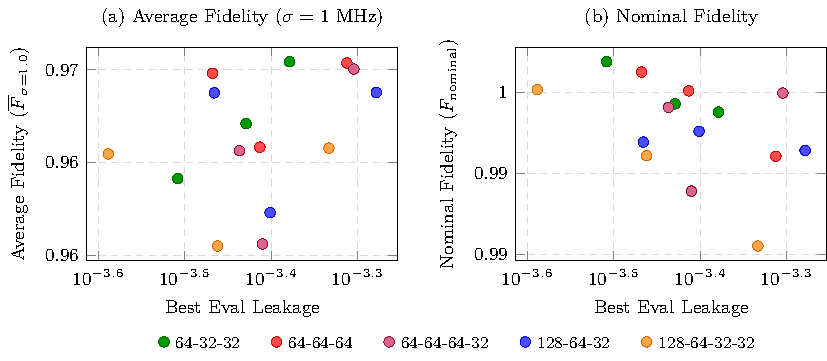
\includegraphics[width=\columnwidth]{architecture_sweep_pareto_combined.pdf}
\caption{Architecture trade-offs: evaluation leakage against (a) average fidelity at $\snoise=1\MHz$
and (b) nominal fidelity. Leakage minimization is not a proxy for robustness --- the layout with the
lowest leakage, $(128,64,32,32)$, has the worst aggregate cost and the weakest robustness.}
\label{fig:archpareto}
\end{figure}

Two conclusions follow. First, architecture is not neutral: moderate changes in width and depth
produce measurable differences in the final trade-off. Second, the dependence is not monotonic. The
deepest model tested achieves the \emph{lowest} mean leakage of the sweep and simultaneously the
\emph{worst} aggregate cost, the weakest robustness and the lowest nominal fidelity
(Fig.~\ref{fig:archpareto}). Minimizing one term of a multi-objective cost is not a selection
principle.

The best aggregate performer is $(64,64,64)$, but its margin over the paper layout $(64,32,32)$ is
$0.2\%$ in evaluation cost, well inside the seed-to-seed spread: the three seeds of $(64,32,32)$ alone
reach $\Fbar_{\sigma=1}=0.959$, $0.962$ and $0.965$. We therefore retain the paper architecture
$(64,32,32)$ for all production runs, which maximizes comparability with Ref.~\cite{Niu2019}. The same
spread sets the resolution of every single-seed comparison in the paper: differences of a few $10^{-3}$ in
$\Fbar$ at $1\MHz$ between two individual runs are not significant on their own.

\subsection{Sensitivity to the UFO weights}
\label{sec:weights}

The weights in Eq.~\eqref{M-eq:ufo} are part of the physical definition of the problem, not optimizer
settings, so they deserve separate treatment. We swept
$\chi\in\{5,10,20\}$, $\mu\in\{0.1,0.2,0.4\}$, $\kappa\in\{0.05,0.1,0.2,0.4\}$ at fixed $\beta=10$
($36$ configurations, two seeds each, five iterations of $10\,000$ episodes with stopping cost $0.15$).
Holding $\beta$ fixed makes the sweep a study of the ratios
$\chi/\beta$, $\mu/\beta$, $\kappa/\beta$, which is the physically meaningful reading and keeps the
design tractable.

\begin{figure}[t]
\centering
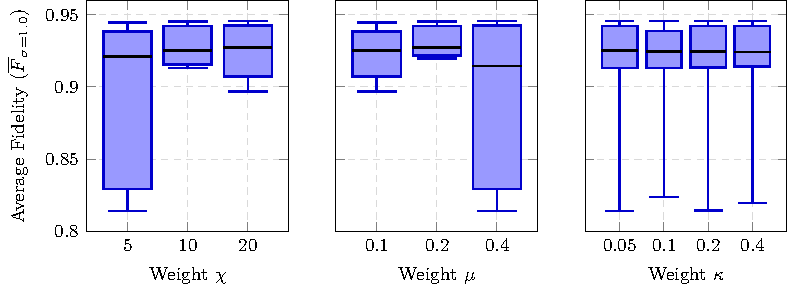
\includegraphics[width=\columnwidth]{ufo_weight_sweep_robustness.pdf}
\caption{Sensitivity of the average fidelity at $\snoise=1\MHz$ to the UFO weights, shown separately
for the fidelity weight $\chi$, the boundary weight $\mu$ and the runtime weight $\kappa$. Underweighting
fidelity ($\chi=5$) opens a failure mode near $\Fbar\approx0.82$; $\mu=0.4$ is strongly bimodal;
$\kappa$ has almost no effect in this fixed-horizon regime.}
\label{fig:ufoweights}
\end{figure}

A methodological caveat governs the whole sweep: the best evaluation cost is \emph{not} a valid
selection criterion across configurations, because different weights define different scalarizations
and their numerical costs are not commensurable. Since all runs here terminate at the same evaluation
time of $180\ns$, increasing $\kappa$ mostly adds a rigid offset. We therefore compare on physical
quantities only --- nominal fidelity, leakage, and robustness at $\snoise=1\MHz$.

The fidelity weight has the clearest effect (Fig.~\ref{fig:ufoweights}). At $\chi=5$ the distribution
is broad and several runs collapse to $\Fbar\approx0.81$--$0.83$; at $\chi=10$ and $\chi=20$ it tightens
around $0.92$--$0.95$. Underweighting logical accuracy relative to leakage lets the optimizer settle
for controls that are clean but simply not the right gate. The boundary weight behaves
non-monotonically: $\mu=0.2$ gives the best median trade-off, $\mu=0.1$ leaves slightly more leakage,
and $\mu=0.4$ becomes strongly bimodal, producing both some of the best runs of the sweep and its worst
lower-tail failures. Larger $\mu$ does reduce the leakage proxy on average --- the lowest-leakage region
is often at $\mu=0.4$ --- but this does not translate into better robust control, which is the same
lesson the architecture sweep taught. The runtime weight $\kappa$ is nearly inert here, for the
structural reason noted above; its influence reappears in Sec.~\ref{M-sec:runtime}, where gate duration
is the observable rather than a fixed boundary condition.

The Pareto-favourable region is occupied jointly by $(\chi,\mu)\approx(10,0.2)$ and
$(\chi,\mu)\approx(20,0.4)$, with the latter marginally ahead. Given two seeds and a small budget, that
margin does not justify departing from the reference scalarization, so we retain the weights of
Eq.~\eqref{M-eq:weights} throughout.

\section{Horizon sweep of the direct optimizer}
\label{supp:horizon}

\begin{figure}[t]
\centering
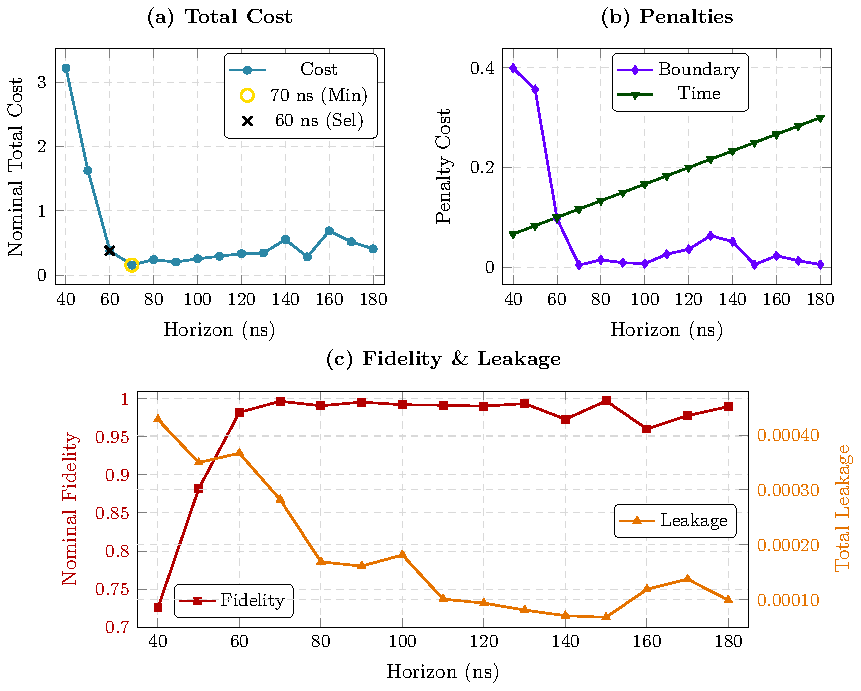
\includegraphics[width=\columnwidth]{adam_single_target_horizon_sweep.pdf}
\caption{direct optimizer on $\Ntgt{2.2}{\pi/2}$ versus gate horizon. (a) Nominal total cost, with the
optimum at $70\ns$ and the pulse selected by the noisy objective at $60\ns$ both marked. (b) Boundary
and runtime penalties. (c) Nominal fidelity and total leakage. The optimum arises from the
simultaneous collapse of the boundary term and the rise in fidelity; longer horizons saturate in
fidelity and are penalized by runtime.}
\label{fig:adamsweep}
\end{figure}

The direct optimizer is trained under noise, but its pulses are compared in the deterministic simulator.
Under that re-evaluation the best horizon is $T^\star=70\ns$, with nominal cost $0.1576$, fidelity
$0.99662$ and leakage $2.82\times10^{-4}$. The optimizer's own noisy objective selects $60\ns$ instead, a
pulse with cost $0.3806$, fidelity $0.98205$ and leakage $3.67\times10^{-4}$; Appendix~\ref{M-app:leak}
explains why it prefers the shorter horizon.

The horizon dependence (Fig.~\ref{fig:adamsweep}) shows what sets the optimum. Below $60\ns$ the pulses
fail, with fidelity $0.73$ at $40\ns$ and $0.88$ at $50\ns$, although their leakage stays in the
$10^{-4}$ range: under strong time compression a pulse cannot be both accurate and zero at its ends, and
it is the boundary term, not the leakage, that grows. Between $60$ and $70\ns$ that term collapses and the
cost falls from $0.381$ to $0.158$. Longer pulses are slightly more accurate and less leaky (fidelity
$0.9971$ at $150\ns$) but pay for it in runtime, so the optimum is the best-balanced pulse and not the
most accurate one. The $70\ns$ pulse is $3.1$ times faster than the generic compiled reference of
Eq.~\eqref{M-eq:tsyn} and $2.1$ times faster than the two-CNOT synthesis of Eq.~\eqref{M-eq:tsyntgt}.

\section{The two family sweeps, target by target}
\label{app:curriculum}

Table~\ref{tab:runtime} lists the curriculum sweep of Sec.~\ref{M-sec:runtime}, and
Fig.~\ref{fig:adamfamily} shows the independent sweep of the direct optimizer.

\begin{table}[t]
\caption{Curriculum runtime sweep over $\Ntgt{\alpha}{\pi/2}$. $\varepsilon=\alpha-\pi/2$ is the
exchange angle of Eq.~\eqref{M-eq:exchange} and $T$ the final evaluation runtime; the last two columns give
the speedup over the generic reference, $215\ns$, and over the target-specific synthesis time of
Eq.~\eqref{M-eq:tsyntgt}, $150\ns$ for every row shown. Rows marked $\dagger$ did not converge (final cost
above $0.40$): their rollouts run to the $180\ns$ ceiling and no speedup is quoted. The row marked
$\ddagger$ is the identity target.}
\label{tab:runtime}
\footnotesize
\begin{ruledtabular}
\begin{tabular}{rrrccrr}
$\alpha$ & $\varepsilon$ & $T$ (ns) & $F^{\mathrm{nom}}$ & $\Fbar_{\sigma=1}$ & $215/T$ & $\Tsyn^{\mathrm{tgt}}/T$\\
\colrule
$0.000^\dagger$ & $-1.571$ & 180 & 0.5577 & 0.6133 & --- & ---\\
$0.157$ & $-1.414$ & 142 & 0.9880 & 0.9510 & 1.51 & 1.06\\
$0.314$ & $-1.257$ & 140 & 0.9905 & 0.9533 & 1.54 & 1.07\\
$0.471^\dagger$ & $-1.100$ & 180 & 0.9538 & 0.9179 & --- & ---\\
$0.628^\dagger$ & $-0.943$ & 180 & 0.9480 & 0.9149 & --- & ---\\
$0.785^\dagger$ & $-0.786$ & 180 & 0.9492 & 0.9055 & --- & ---\\
$0.942$ & $-0.629$ & 148 & 0.9905 & 0.9504 & 1.45 & 1.01\\
$1.099$ & $-0.472$ & 76 & 0.9850 & 0.9674 & 2.83 & 1.97\\
$1.256$ & $-0.315$ & 140 & 0.9894 & 0.9535 & 1.54 & 1.07\\
$1.413$ & $-0.158$ & 132 & 0.9880 & 0.9542 & 1.63 & 1.14\\
$1.570^\ddagger$ & $-0.001$ & 2 & 0.99999 & 0.9994 & --- & ---\\
$1.727$ & $0.156$ & 124 & 0.9861 & 0.9575 & 1.73 & 1.21\\
$1.884$ & $0.313$ & 108 & 0.9821 & 0.9582 & 1.99 & 1.39\\
$2.041$ & $0.470$ & 106 & 0.9825 & 0.9595 & 2.03 & 1.42\\
$2.198$ & $0.627$ & 110 & 0.9837 & 0.9545 & 1.95 & 1.36\\
$2.355$ & $0.784$ & 118 & 0.9863 & 0.9573 & 1.82 & 1.27\\
$2.512$ & $0.941$ & 136 & 0.9919 & 0.9567 & 1.58 & 1.10\\
$2.669$ & $1.098$ & 144 & 0.9918 & 0.9547 & 1.49 & 1.04\\
$2.826^\dagger$ & $1.255$ & 180 & 0.9340 & 0.8944 & --- & ---\\
$2.983^\dagger$ & $1.412$ & 180 & 0.9213 & 0.8872 & --- & ---\\
$3.140^\dagger$ & $1.569$ & 180 & 0.9400 & 0.9020 & --- & ---\\
\end{tabular}
\end{ruledtabular}
\end{table}

\begin{figure}[t]
\centering
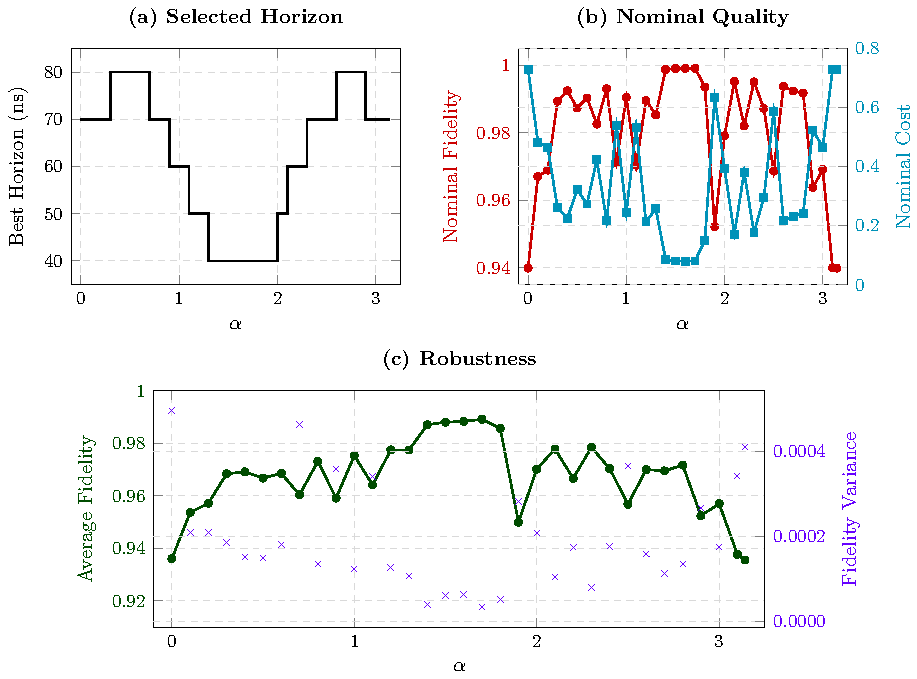
\includegraphics[width=\columnwidth]{adam_family_sweep.pdf}
\caption{No-transfer control: the direct optimizer swept independently over $33$ targets of
$\Ntgt{\alpha}{\pi/2}$. (a) Selected horizon versus $\alpha$. (b) Nominal fidelity and cost.
(c) Average fidelity at $\snoise=1\MHz$ and the corresponding variance. The horizon is shortest around the
identity target $\alpha=\pi/2$ and grows with the exchange angle $|\alpha-\pi/2|$.}
\label{fig:adamfamily}
\end{figure}

\section{Relation to hardware}
\label{supp:hardware}


This paper compares optimizers on a common model, and none of its fidelities is a statement about a
device. Five remarks place that model against current hardware.

\emph{Noise.} Frequency and amplitude noise in superconducting circuits is dominated by low-frequency
components --- $1/f$ flux and charge noise and slow drift of the calibration~\cite{Krantz2019,Paladino2014}.
Of the noise models of Sec.~\ref{M-sec:robust} the quasi-static one is therefore the closer to a device, and
the white model of Ref.~\cite{Niu2019}, under which no training can help, the further.

\emph{Decoherence.} The model is closed. Weak relaxation and pure dephasing, at rates $\Gamma_1=1/T_1$ and
$\Gamma_\varphi=1/T_\varphi$ on each qubit, lower the average fidelity of any two-qubit gate of duration
$T$ by $\tfrac{4}{5}T(\Gamma_1+\Gamma_\varphi)$, whatever the gate~\cite{Abad2022}: like white control
noise, Markovian decoherence leaves a pulse nothing to exploit but its duration. For
$T_1=T_\varphi=100\,\mu\mathrm{s}$, of the order of current processors~\cite{GoogleQAI2025}, this is
$1.1\times10^{-3}$ for the $70\ns$ pulse of the direct optimizer and $1.9\times10^{-3}$ for the $116\ns$ pulse of the noise-free agent,
comparable to the nominal infidelities of Table~\ref{M-tab:single}. By the same formula the white noise of
the model at $1\MHz$ costs as much as $T_1=T_\varphi\approx5\,\mu\mathrm{s}$, and the runtime weight of
Eq.~\eqref{M-eq:ufo} corresponds to $T_1=T_\varphi\approx12\,\mu\mathrm{s}$. Both describe devices an order
of magnitude less coherent than today's; a weight matched to current coherence would move the optimum of
Eq.~\eqref{M-eq:ufo} towards longer and more accurate pulses.

\emph{Bandwidth.} The $10\MHz$ filter is narrow by hardware standards. Sycamore processors, descendants of
the gmon, drive single-qubit gates with $25\ns$ pulses and perform iSWAP-like gates by turning on a
$20\MHz$ coupling for $12\ns$~\cite{Arute2019}: the amplitude bound of the present model, four to six
times faster than the $54$--$72\ns$ that its filter allows for the same exchange angle
(Sec.~\ref{M-sec:physicalinterp}). The runtimes of Sec.~\ref{M-sec:runtime} are thus set by a modelling choice
of Ref.~\cite{Niu2019} more than by the coupler.

\emph{Higher levels.} Those fast gates are not members of the benchmark family. The coupling shifts
$\ket{11}$ through $\ket{02}$ and $\ket{20}$ by $4g^2/|\eta|$, so an exchange pulse carries a conditional
phase $\phi=(4/|\eta|)\int g^2dt$, which $\Ntgt{\alpha}{\pi/2}$ does not contain and local rotations
cannot remove; an otherwise perfect pulse is left with $1-F=\sin^2(\phi/4)$. This is what limits the
pulses optimized without noise in Sec.~\ref{M-sec:memory}, whose nominal infidelities equal
$\sin^2(\phi/4)$ to within $1\%$. In this model the fidelity of an exchange pulse therefore improves only
as $1/T^2$, a trade-off that native gate sets avoid by making $\phi$ part of the gate~\cite{Foxen2020} or
by cancelling it through the level structure of the coupler~\cite{Sung2021}.

\emph{Absolute fidelity.} Two-qubit gates on tunable-coupler transmons reach a Pauli error of
$3.8\times10^{-3}$ for a continuous fSim family on gmon qubits~\cite{Foxen2020}, and fidelities of
$99.76\%$ and $99.87\%$ for CZ and iSWAP gates~\cite{Sung2021}, decoherence included. The closed-system
fidelities of Table~\ref{M-tab:single} are not competitive pulse designs and are not offered as such: what
transfers from this study is the comparison between methods and the two structural results of
Sec.~\ref{M-sec:conclusion}.

\bibliographystyle{apsrev4-2}
\bibliography{references}

\end{document}
